\section{Results}
\subsection{Baseline: The Connectome Is a Specific, Low-Latency Controller}
Driving LC4 and LPLC2 at 150\,Hz produces a command-population rate of $94.7$\,Hz (median over 12 trials; interdecile 94.0--95.6\,Hz) with 4.05\,ms median first-spike latency, far above $\theta$ (Fig.~\ref{fig:baseline}). An equal-sized random set, driven identically, yields only $8.2$\,Hz on the same readout while producing \emph{more} total activity (293k vs.\ 40k spikes): the readout is pathway-specific, not generic arousal. When both sensory channels are silenced (F5\textsubscript{both}), the command rate collapses to exactly zero in every trial while the rest of the brain keeps spiking at background level: the score measures transmission through the instrumented pathway.

\begin{figure}[tb]
\centering
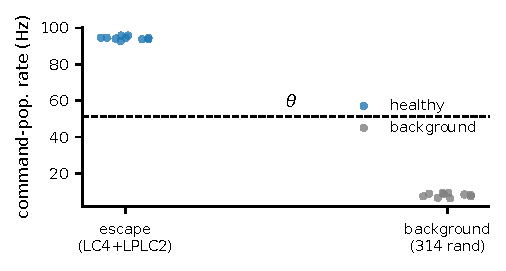
\includegraphics[width=\columnwidth]{figs/fig2_baseline.pdf}
\caption{Readout specificity. Command-population rate under escape stimulation (LC4$+$LPLC2) versus matched random-site stimulation (314 cells); dashed line: $\theta$.}
\label{fig:baseline}
\end{figure}

\subsection{Tolerance Curves: Noise Is Absorbed, Disconnection Degrades Gracefully}
Figure~\ref{fig:curves} shows dose--response curves for the two most consequential families; the F1 and F3 responses are flat in median (Table~\ref{tab:principles}). Weight variability (F1) leaves the median unchanged: at $\sigma{=}0.5$ the rate is $94.2$\,Hz (healthy: 94.7\,Hz) while the trial dispersion widens (interdecile 90.4--100.8 vs.\ 94.0--95.6\,Hz healthy), and total activity rises only from 39.7k to 41.6k spikes. Random synapse deletion (F2) degrades gracefully: 5\% and 10\% loss leave the rate at 91.9 and 93.1\,Hz, 25\% loss retains $84.5$\,Hz (89.2\% of baseline), and even 50\% loss retains $72.4$\,Hz (76.5\%), with all 12 trials passing the transmission criterion in every condition (weakest trials 63.1 and 68.1\,Hz---above $\theta$ by $\geq$22\%). Disconnection's cost appears predominantly in latency: 4.05 to 5.4\,ms at 50\% loss (+33\%), consistent with recruitment of longer residual multi-hop routes; which dominates a task-level error budget is workload-dependent. Random unit loss (F3) up to 10\%---nearly 14{,}000 neurons with all their synapses---leaves the median unchanged (95.1 vs.\ 94.7\,Hz): command drive integrates over hundreds of converging populations, and no tested random 10\% slice is load-bearing. The wide 1{,}299-neuron descending layer tracks the same pattern (2{,}941 spikes healthy vs.\ 1{,}918 at 50\% loss), so the graded response is a property of command encoding, not of the eight-neuron readout.

\begin{figure*}[tb]
\centering
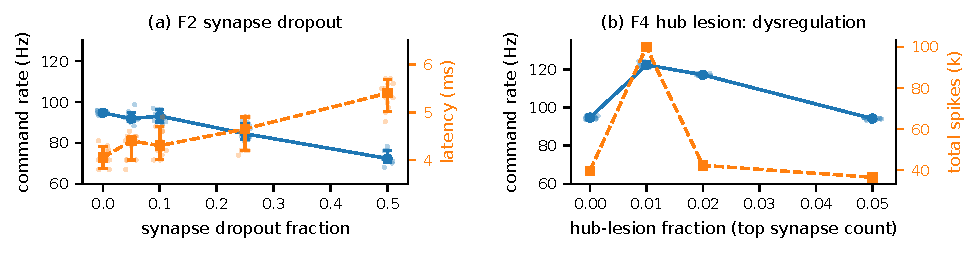
\includegraphics[width=\textwidth]{figs/fig3_curves.pdf}
\caption{Behavioral tolerance curves (medians over 12 trials, blue: rate; orange: latency ms (a) / total spikes (b); dots: trials; dotted grey: healthy medians). (a) Synapse dropout: 76\% of the command rate retained at 50\% loss while latency rises 33\%. (b) Hub lesion: dysregulation, not signal loss.}
\label{fig:curves}
\end{figure*}

\begin{figure*}[tb]
\centering
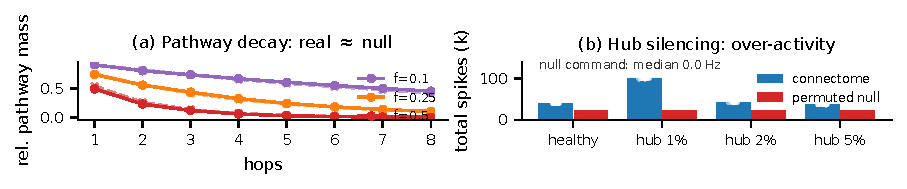
\includegraphics[width=\textwidth]{figs/fig4_topology.pdf}
\caption{Topology contrast. (a) Route mass under edge loss, normalized per graph (solid: connectome, dashed: permuted null): relative decay nearly identical, absolute mass 5.8--17.7$\times$ higher. (b) Activity under hub lesions: runaway only in biological wiring; null command readout at 0.0\,Hz.}
\label{fig:topology}
\end{figure*}

\subsection{Hub Loss Produces Runaway, Not Silence}
The dose--response of hub removal (F4) is non-monotonic and qualitatively different from every distributed fault (Figs.~\ref{fig:curves}b, \ref{fig:topology}b). Removing the top 1\% of cells ranked by total outgoing synapse count (1{,}386 neurons, 9.1\% of all connections) \emph{increases} the command rate to $122.3$\,Hz (+29\%, interdecile 121.1--123.9\,Hz across trials) and more than doubles global activity (99.9k spikes, $2.52\times$ healthy; Mann--Whitney vs.\ healthy $p<10^{-4}$, as for F2$_{50}$ and F5$_{\mathrm{both}}$); at 2\% the rate stays elevated (117.1\,Hz) with activity partially normalized (42.4k); at 5\% (22.4\% of connections) both metrics return to near-baseline (94.2\,Hz, 36.4k). A matched-scale contrast shows this is not a size effect: random 10\% unit ablation disconnects 10.0\% of connections (more than the hub set's 9.1\%) yet leaves the readout unchanged (95.1\,Hz). Hub lesions do not starve the pathway of drive---they remove broadly connected inhibitory regulation, and spared circuitry over-drives the command layer: about 62\% of removed hub output connections are inhibitory, versus 40\% network-wide. We therefore score \emph{transmission} (rate $\geq\theta$) and an \emph{activity envelope} (rate and total activity within $2\times$ of healthy) separately: hub loss at 1\% passes transmission in all trials while violating the envelope in all 12 (the violation persists for any envelope multiplier between $1.5\times$ and $2\times$); every distributed fault passes both; F5\textsubscript{both} fails both. The envelope violation is the engineered system's dangerous mode: output exceeds its envelope while every per-unit monitor reads ``active.'' The same lesion in the permuted null produces no such signature, tying the runaway to biological hub structure, not degree heterogeneity per se.

\subsection{What the Wiring Contributes: Null Network and Pathway Analysis}
The permuted null dissociates specificity from redundancy: out-degrees, weights, and the in-degree histogram survive, convergence is reassigned, and the null transmits \emph{nothing} to the command layer (0.0\,Hz in every condition and trial); its broad 1{,}299-neuron readout falls to background (45.5 spikes per trial vs.\ 2{,}941 healthy) and global activity to about 60\% of the biological level (23.8k vs.\ 39.7k)---it spikes, but nothing converges onto descending output. Pathway mass quantifies the convergence advantage: 5.8$\times$ more 1-hop and 17.7$\times$ more 4-hop route mass from sensory input into the descending layer than the null. Yet \emph{relative} pathway-mass decay under the same deletion levels is nearly identical in both graphs (at $f{=}0.5$, $k{=}8$: 0.3\% vs.\ 0.4\% of baseline; Fig.~\ref{fig:topology}a). Combined with behavior degrading far more slowly than pathway mass (76\% functional retention at $f{=}0.5$ against 5.8\% four-hop route mass), this rules out graph redundancy alone and is consistent with a threshold-amplification account of the topological-to-functional conversion. The comparison does not isolate the dynamics by itself: the 594 direct sensory$\to$DN connections, which survive edge deletion in proportion, and excitation--inhibition rebalancing could contribute; targeted controls are needed. A threshold-amplification account is simple: with $N$ afferents converging and per-synapse survival $p$, converged drive scales as $Np$ while $k$-hop route mass decays as $p^k$ (6.25\% at $k{=}4$, $p{=}0.5$); the threshold's saturating nonlinearity maps drive onto output, so the rate retains 76.5\% at $p{=}0.5$ and 89.2\% at $p{=}0.75$, above the linear 50\% and 75\% bounds the account predicts; near-threshold drive is where it should fail, saturation compressing increases more than decreases. Graceful degradation here reflects convergent wiring preserving aggregate drive plus threshold dynamics compressing drive changes into small rate changes.

